\vspace*{-5mm}
\mysection{Architectural Design}

\mysubsection{Overview}
In this chapter we will analyze the proposed architecture and components of Travlendar+ system.\par
The proposed architecture is composed by three tiers :
\begin{itemize}
	\setlength{\leftskip}{0.5cm}
	\item \emph{Presentation Tier : }it's represented by the Browser and the Mobile App, the View part of our system.
	\item \emph{Web and Business Tier : }it's represented by the Web Server, which responds to the user's HTTP requests, and the Application Server, which contains all the Business Logic.
	\item \emph{Database Tier : }it's represented by the DB Server, that contains and manages persistent data in an efficient way.
\end{itemize}
\begin{figure}[H]
	\centering
	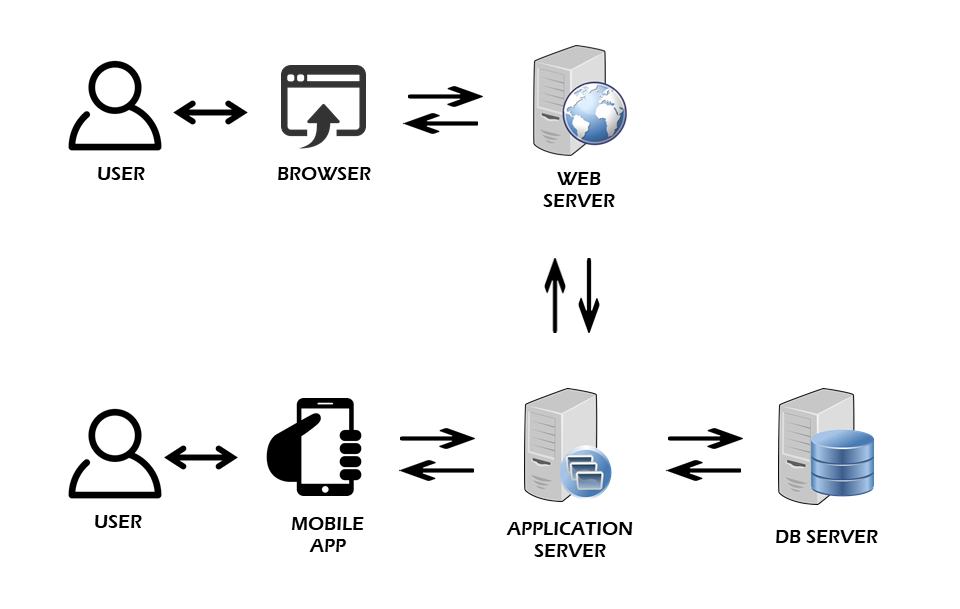
\includegraphics[scale=0.35]{Images/Architecture/Proposed_Architecture}
	\caption{Proposed Architecture}
\end{figure}

\mysubsection{High Level Components and Their Interactions}
\begin{figure}[H]
	\centering
	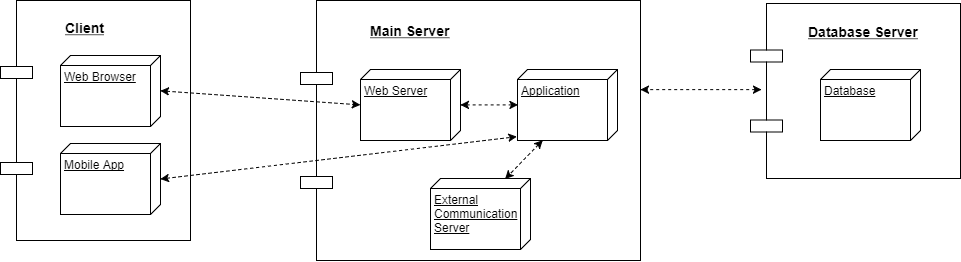
\includegraphics[scale=0.35]{Images/Architecture/Components_High_Level}
	\caption{Components High Level}
\end{figure}

The system is divided in three main layers: Presentation Layer, Business Layer and Data Layer.
The presentation layer is both a web-based application and a mobile application. For the web application we will have a very thin client with the only aim of performing requests, through a web server, to the Business layer and receiving the HTML pages with the demanded information.
On the other hand, the mobile application will not require an interface with the web server because it will communicate directly with the server.

The main server is composed by three parts : the Web Server, mentioned here above, the Application and the External Communication Server. The application part of the main server contains all the system's logic: it receives requestes and input data from the client side and performs all the necessary operations.
The External Communication Server part is in charge to handle all the comunication with the external services to retrieve data of interests from other systems in order to achieve the system goals.
Our system, being a calendar based application, will have the main issue of managing a richly structured body of information. In our case, this information will be persistently stored in multiple Data Bases, each one containing a precise schema with a precise kind of data, and they always have to reflect the true state of affairs. For this reason, every client request, implicating a changing data operation is preceded by a set of controls performed by the Business logic in order to maintain the database’s consistency.

\mysubsection{Component View}
\begin{figure}[H]
	\centering
	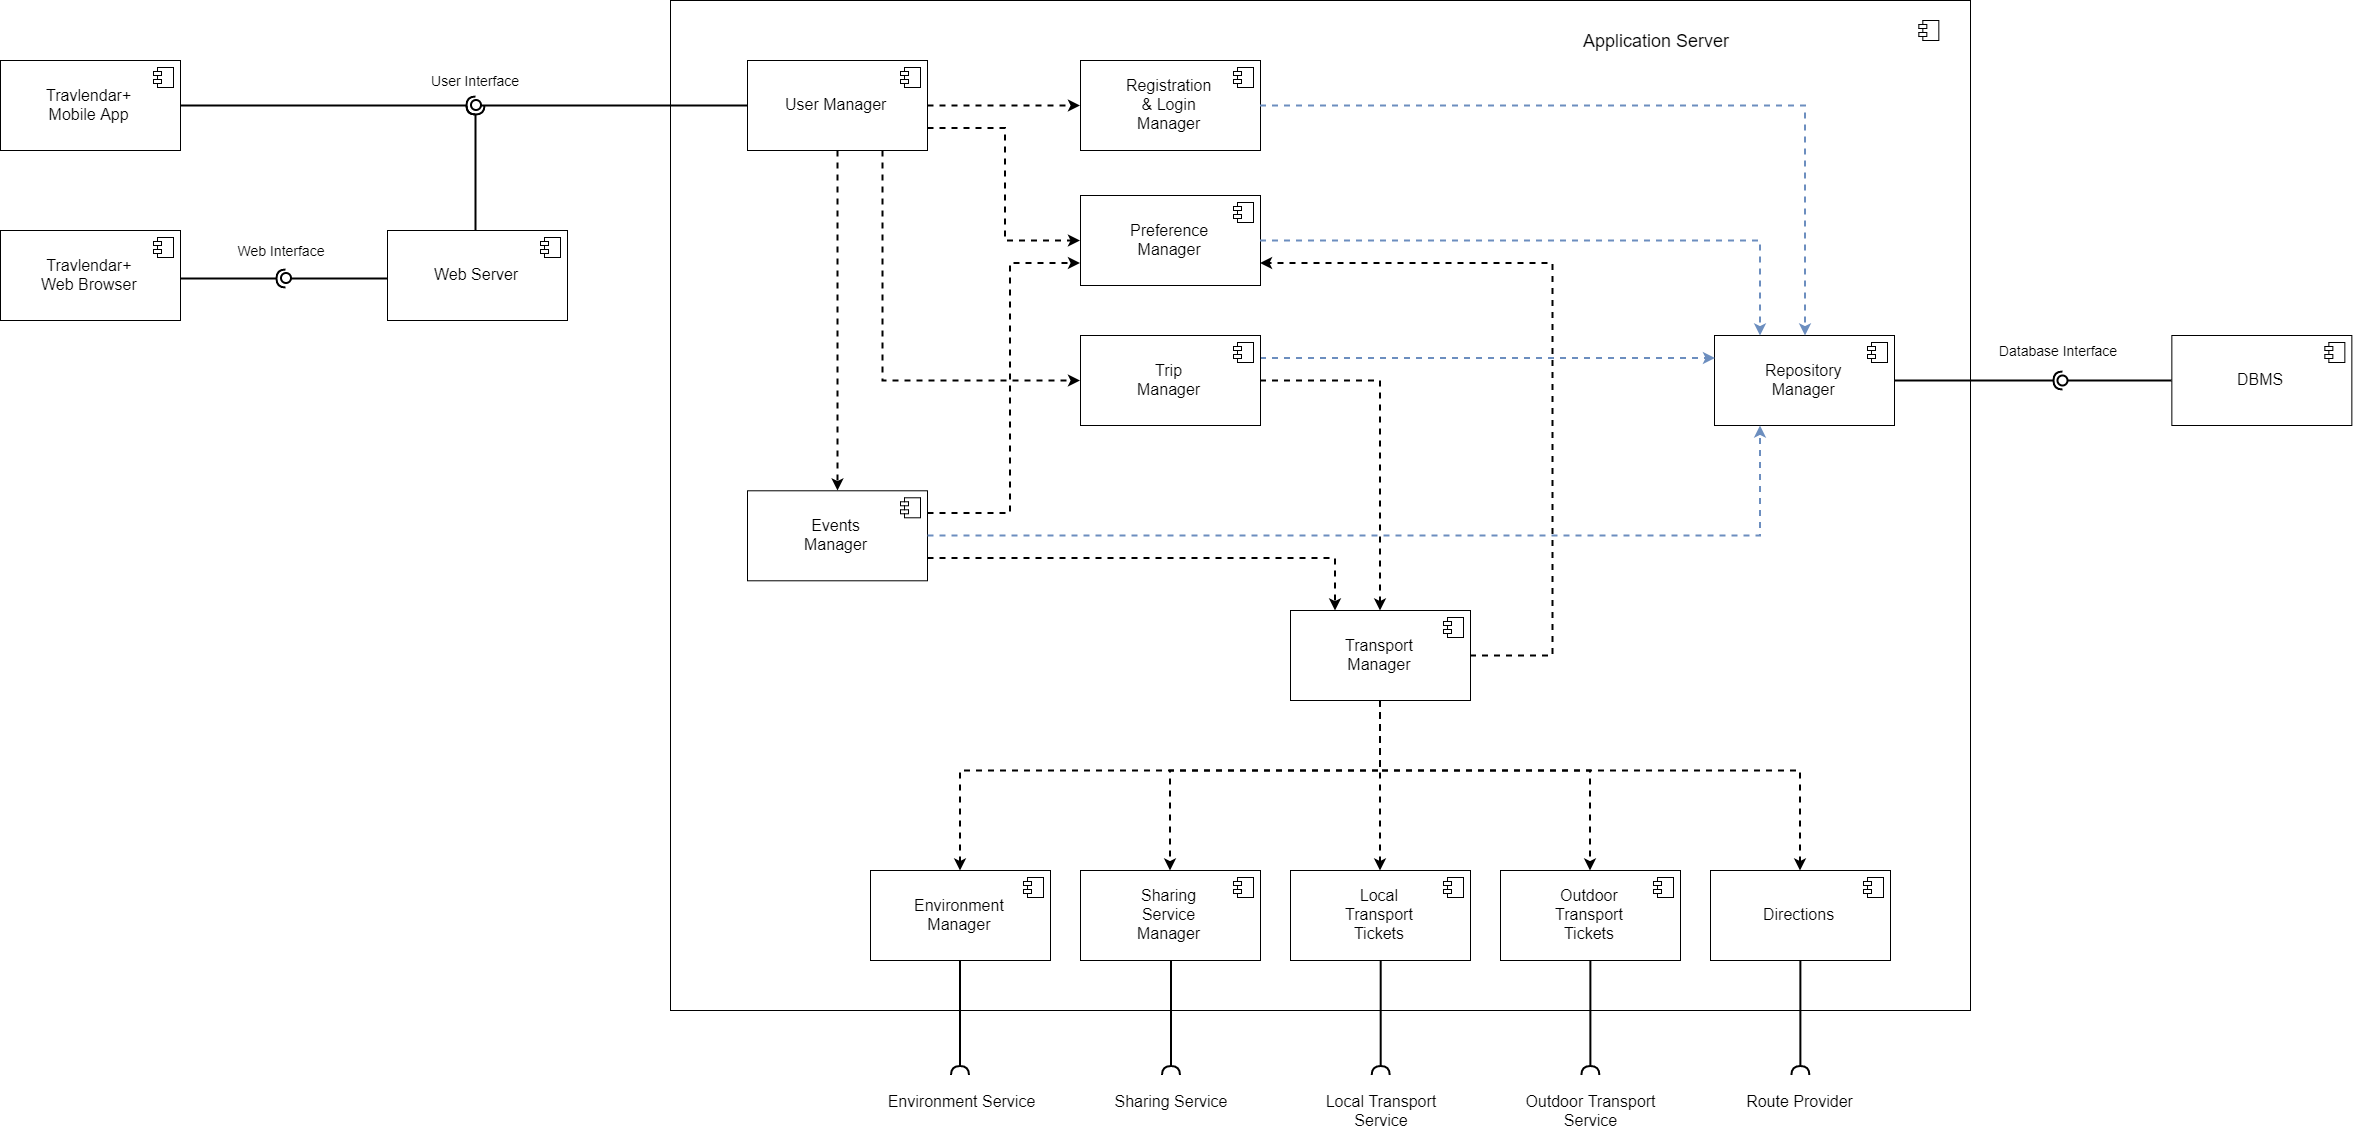
\includegraphics[scale=0.17]{Images/Architecture/Components_View}
	\caption{Component View}
\end{figure}
\mysubsubsection{Travlendar+ Mobile App}
This is the component responsible for the communication between user devices, i.e. smartphone, and the rest of the system. It will exchange REST messages with the \emph{userInterface} and rendering the UI based on the server replies.\par
In order to communicate with the server the component will use specific frameworks and libraries depending on the specific device used by the user (i.e. Android SDK Platform for Android smartphones).\par
This component represents the View part of our MVC pattern.

\mysubsubsection{Travlendar+ Web Browser}
This is the component responsible for the communication between the user browser and the rest of the system.\par
It sends HTTP requests to the \emph{webInterface} in order to get back from the server HTML pages and static resources like CSS and JavaScript files.

\mysubsubsection{Web Server}
This component is responsible for the HTTP responses of the \emph{webInterface}. Its main function is to elaborate pages, generate contents dynamically and send them back to the browser. These processes are performed by the Web Server instead of the user Browser to manage efficiently the user CPU load.\par
An example could be the Apache HTTP Server. It’s a cross-platform server, highly scalable, that using a \emph{gzip} module reduces web pages size (weight).

\mysubsubsection{User Manager}
This is one of the most important server component that handles the communication with the user and takes care of all possible breakouts and errors that may occur at runtime. It also manages all user requests redirecting them to other server specific components.

\mysubsubsection{Registration \& Login}
It allows the user to register and log into the system, memorizing and verifying user credentials.

\mysubsubsection{Preference Manager}
It allows the user to set all his preferences, such as carbon footprint, TAGs, residence location, etc… with the purpose to memorize these data in the DB through the Repository Manager and retrieve them whenever it's needed.

\mysubsubsection{Trip Manager}
This component handles all user trips, allowing him to add, delete or edit them. It also allows the user to buy tickets to reach the trip location (through the Outdoor Transport Tickets component) and the ones for local transport services in the destination city (through the Local Transport Tickets).

\mysubsubsection{Events Manager}
This component takes care of user calendar, managing the events that he wants to add, delete, edit or visualize.\par
Thus, anytime he can :
\begin{itemize}
	\setlength{\leftskip}{1cm}
	\item \emph{insert or edit an event :} the component will check through the Repository Manager if in the DB there is an overlap and if the event is reachable from the previous one (using also Transport Manager to verify route time).
	\item \emph{delete an event :} the component will simply delete it in the DB.
	\item \emph{visualize an event :} the component will check through the Transport Manager the available means of transport, the time needed and suggest the route to reach the event.
\end{itemize}

\mysubsubsection{Transport Manager}
This component handles all the means of transport and tickets. Concerning transport, it will filter the means according to :
\begin{itemize}
	\setlength{\leftskip}{1cm}
	\item the means selected in the event’s TAG;
	\item the $CO_2$ preference;
	\item the means selected in the “Available Means” in Preferences;
	\item the available means to reach the event (suggested by the route provider);
	\item the weather forecast;
	\item eventual strikes.
\end{itemize}
It allows also to buy local transport tickets, if needed. 

\mysubsubsection{Directions}
This component will handle the communication with the route provider in order to get maps, means and routes to reach a specific destination. To get these information it will use API requests (i.e. Google APIs).
It will also parse and elaborate the API responses in specific structures, ready to be used by the server components when needed.

\mysubsubsection{Environment Manager}
This component will be used by our system to check and warn the user about the weather conditions and eventual transport strikes.
It will use API requests to communicate with the external services.

\mysubsubsection{Sharing Service Manager}
This component will allow our server to communicate with the external sharing services and retrieve the nearest sharing mean of transport GPS position.

\mysubsubsection{Local Transport Tickets}
It will take care of the communication with the local transport services, in order to get information about the available tickets, suggesting the best deal based on his travel needs.

\mysubsubsection{Outdoor Transport Tickets}
It will take care of the communication with the outdoor transport services, in order to get information about the available tickets and means of transport.

\mysubsection{Deployment View}
\textcolor{red}{\Huge INSERISCI TESTO}
\begin{figure}[H]
	\centering
	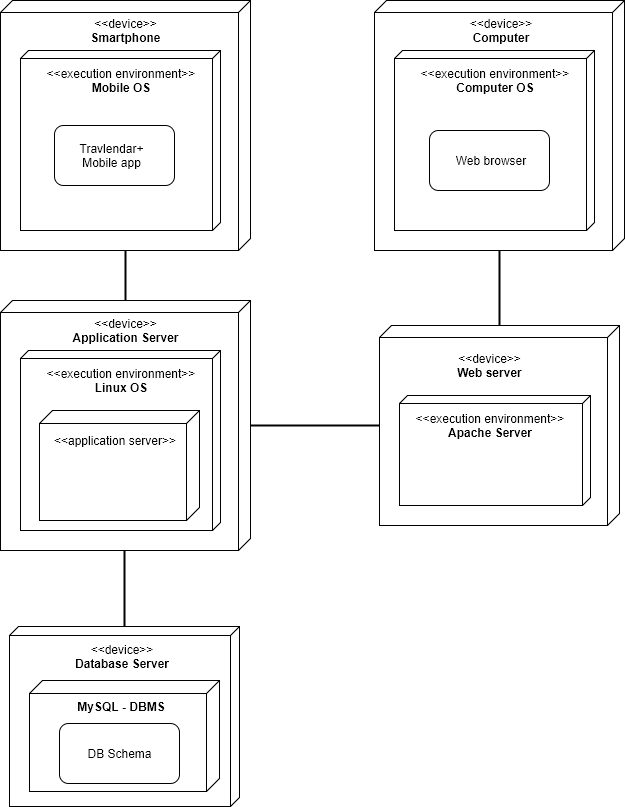
\includegraphics[scale=0.17]{Images/Architecture/Deployment_View}
	\caption{Deployment\_View}
\end{figure}

\mysubsection{DB Structure}

\textcolor{red}{\Huge INSERT DBMS DIAGRAM}

\mysubsection{Runtime View}
In this section we will see some Runtime Views in order to see how the components interact according to specific requests.
For the client-side we have taken into consideration the Web Browser only, in order to evaluate the interaction between the Browser and the Web Server, the Web Server and the Application Server components.

\mysubsubsection{Registration}
This Runtime View shows a user Registration process.\par
First of all the Web Server sends to the user the registration\_form to be fulfilled with his credentials. As soon as the information are inserted, the form is sent back to the Server.\par
At this point, it’s important to check if the email is already associated to another account. In order to do that, the server calls method on the DBMS to retrive this information. If the get\_result it’s equal \emph{Null} the email it’s not used and the server can complete the registration saving in the DB the user credentials. Otherwise, the server will notify the user that the inserted email cannot be used.
\begin{figure}[H]
	\centering
	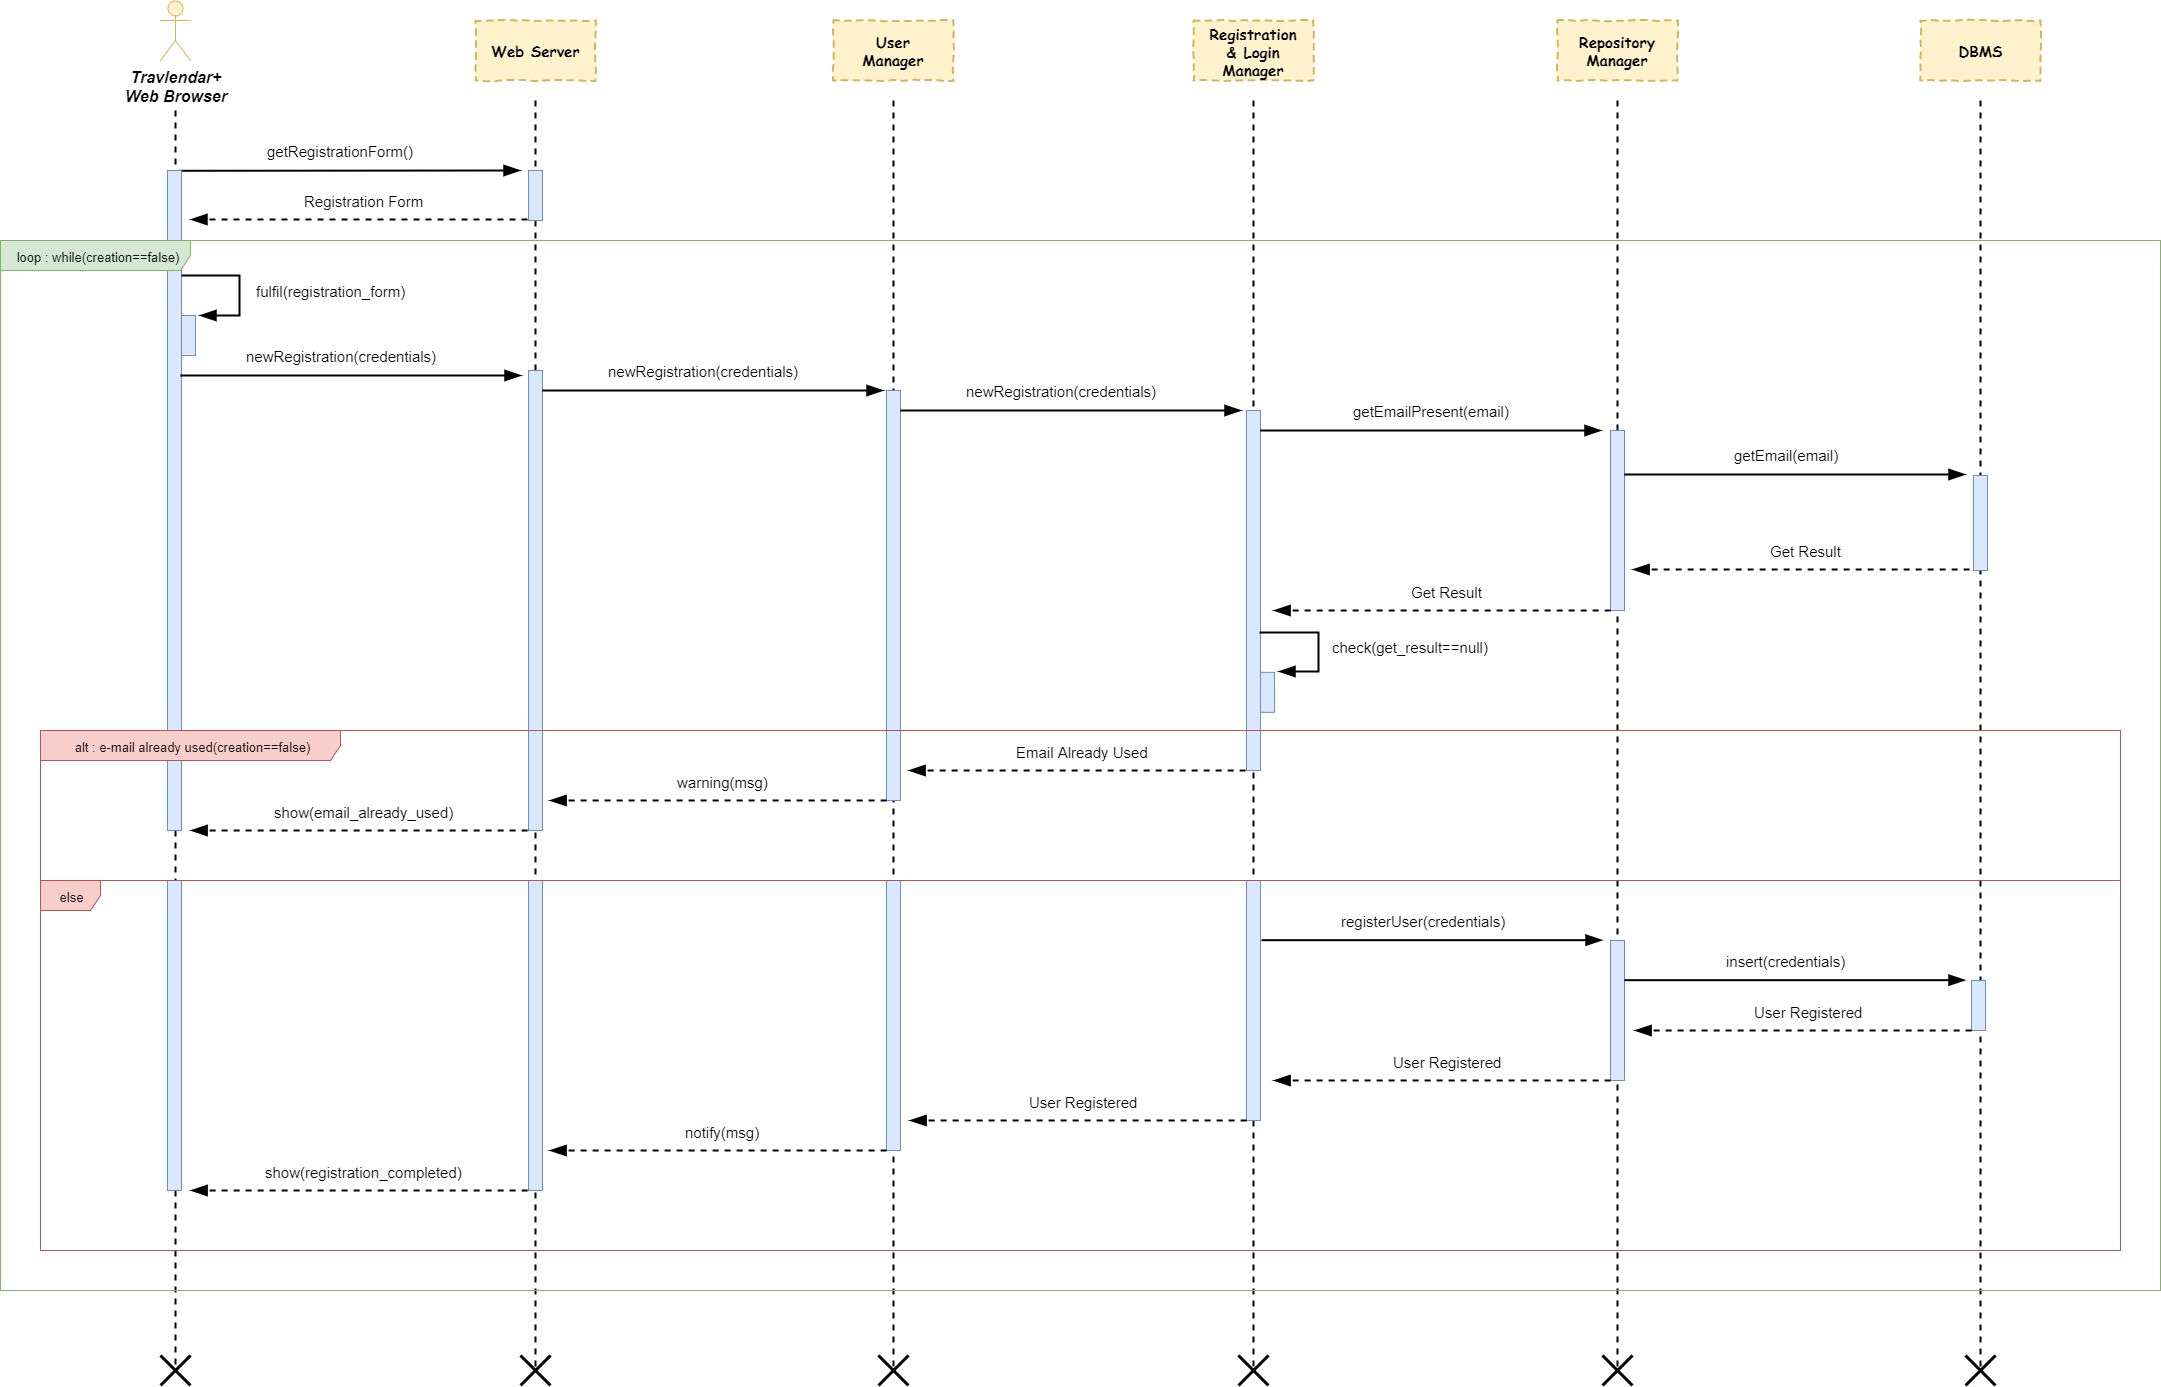
\includegraphics[scale=0.2]{Images/Runtime/Registration}
	\caption{Registration Runtime View}
\end{figure}

\mysubsubsection{Login}
This Runtime View shows a user Login process.\par
As in the previous runtime, the Web Server sends to the user the login\_form to be fulfilled with his credentials. As soon as the information are inserted, the form is sent back to the Server to be checked.\par
First of all it has to check if the user email is present in the DB and then if the user password is correct. In order to accomplish this task in an efficient way, the server asks the DBMS to retrieve him the password related to the inserted email. If the get\_result is equal \emph{Null} there is no account registered with that email. Otherwise, the server, more specifically the Registration \& Login Manager, has to check if the get\_result is equal to the inserted password.
If that check succeeds, then the user is logged and the server gets and shows to the user the events related to the current month retrieved from the DB.
\begin{figure}[H]
	\centering
	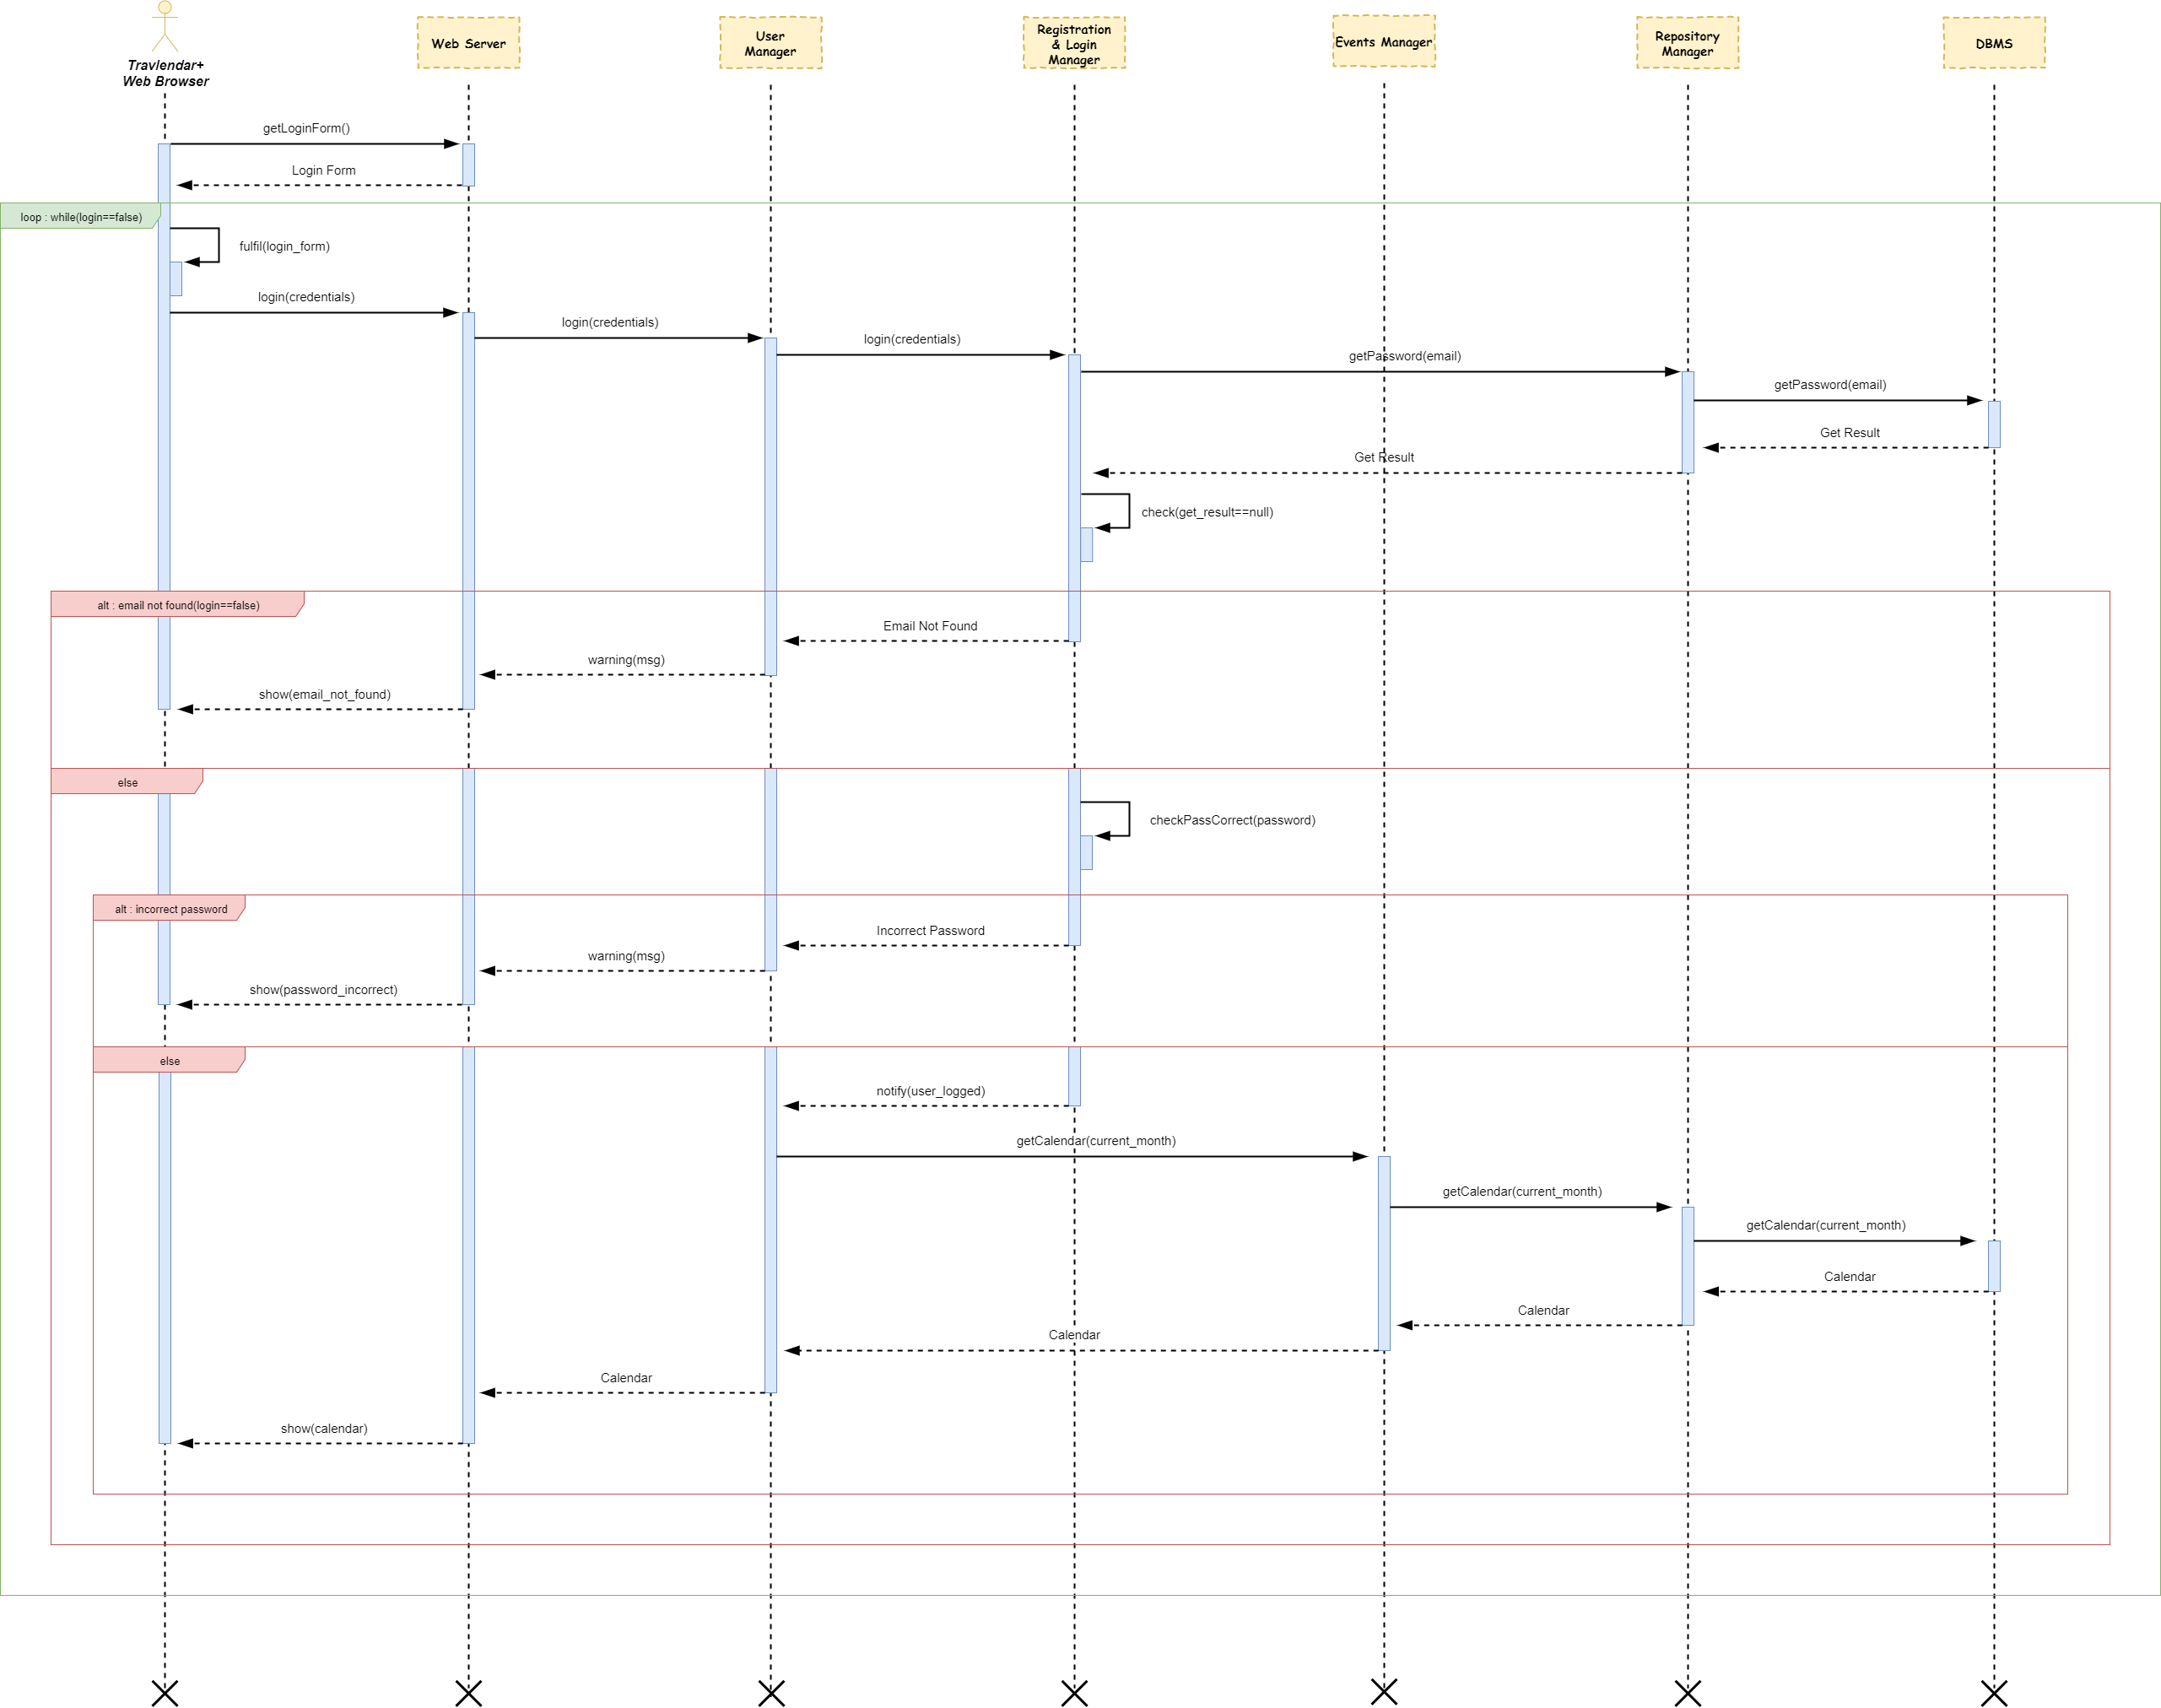
\includegraphics[scale=0.17]{Images/Runtime/Login}
	\caption{Login Runtime View}
\end{figure}

\mysubsubsection{Add Event}
This Runtime View shows the Add Event process.\par
In order to reduce the diagram size we have made some premises :
\begin{itemize}
	\setlength{\leftskip}{1cm}
	\item There is a Previous and a Next Event, before and after the event that the user is adding. In this way we don’t have to show runtime the check that verifies if the getPreviousEvent() or the getNextEvent() is equal to \emph{Null}.
	\item The user hasn’t already configured the lunch preference, so there is no lunch event in the calendar. In this way we don’t have to run the check for verifying that the inserted event overlaps with a lunch event. In fact, if the overlapped event was a Lunch, the system would have to check if it could be moved or reduced respecting the lunch contraints.
\end{itemize}\par
Even in this runtime, firstly the user has to complete the event\_form and send it to the server.
Once Events Manager receives the data, it has to check :
\begin{enumerate}
	\setlength{\leftskip}{1cm}
	\item \emph{If the event Overlaps :} Events Manager asks the Repository Manager to search in the DB if there’s a planned event at the same time of the inserted one. If the get\_result is equal to \emph{Null} there’s no overlap.
	\item \emph{If the event is reachable from the previous one :} Events Manager asks the Repository Manager to get the information of the previous event, especially its location. Once received, it sends both the locations to the Directions Component in order to get the route time. Finally, it checks if the event is reachable or not.
	\item \emph{If the next event is reachable from the inserted one :} it’s like the previous check but it gets from the DB the information of the next event instead of the previous one.
	If all the checks succeed, the server will add the event in the DB and shows it to the user.
\end{enumerate}
\begin{figure}[H]
	\centering
	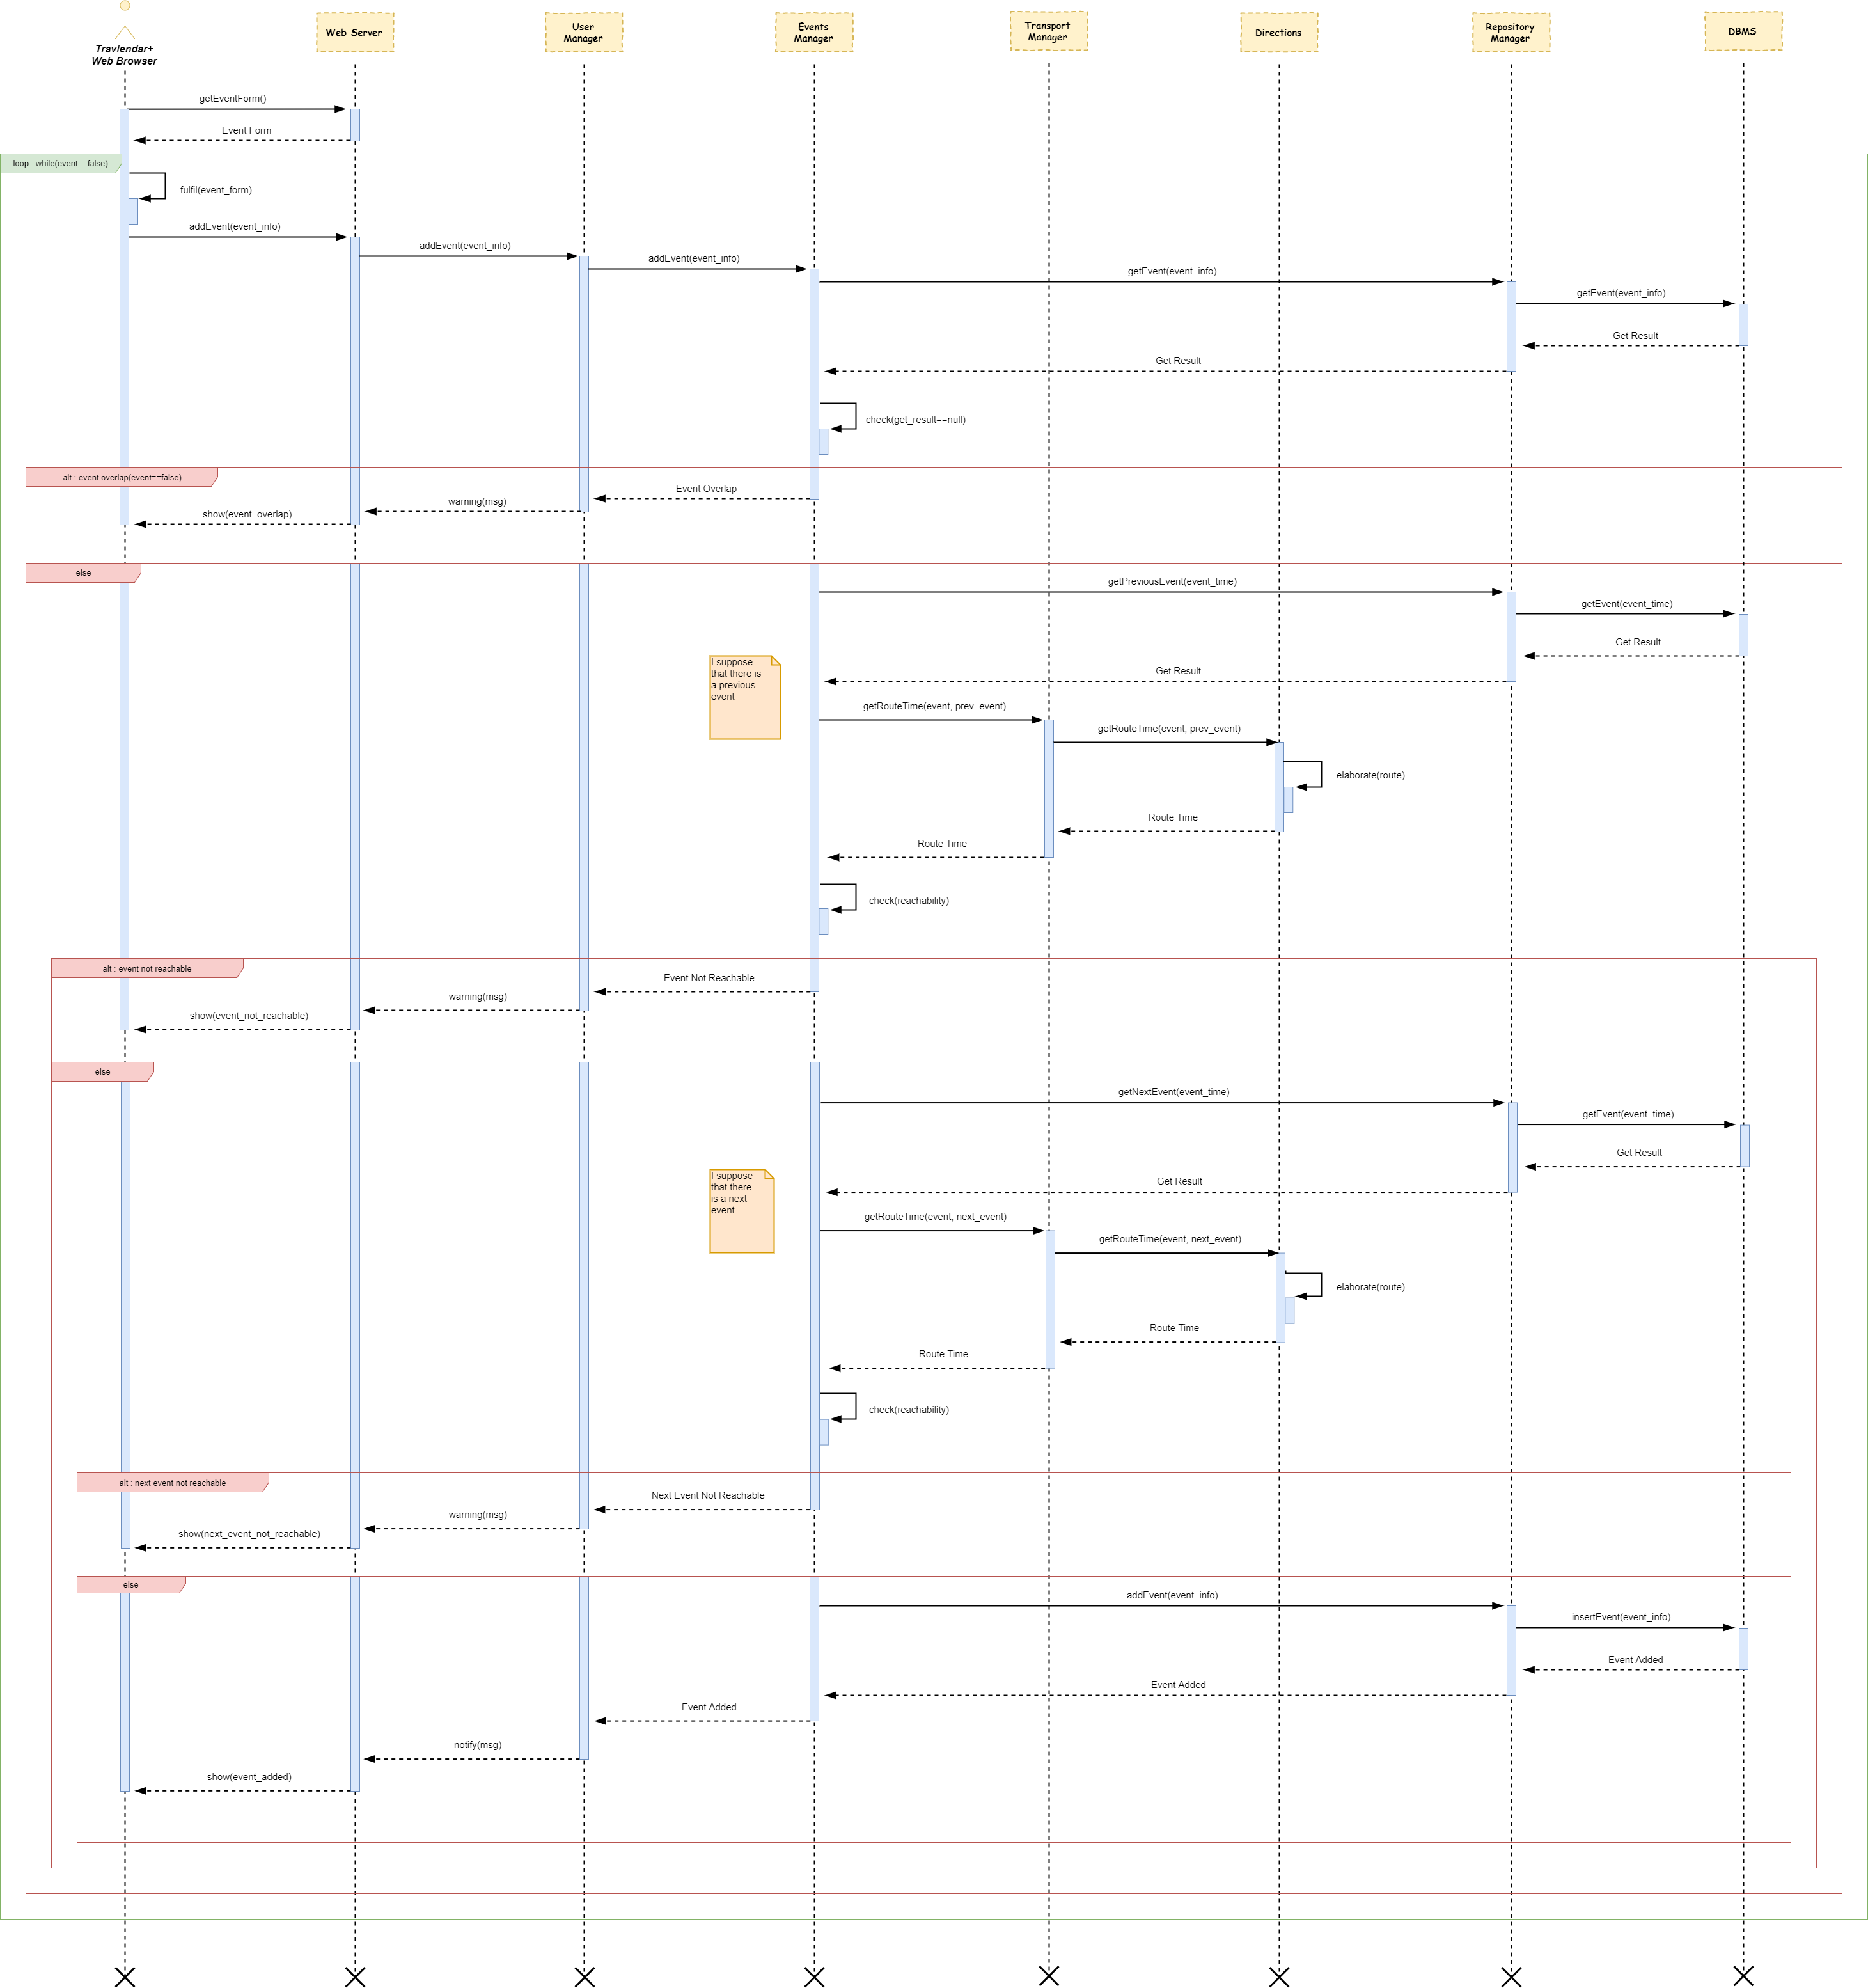
\includegraphics[scale=0.15]{Images/Runtime/Add_Event}
	\caption{Add Event Runtime View}
\end{figure}

\mysubsubsection{Visualize Event}
This Runtime View shows a user's Visualize Event process.\par
In order to reduce the diagram size we make a premise : the system has already checked that there exists an event before the one that the user wants to visualize.\par
In this diagram the user asks the server to show him an event. For achieving this result, the server has to get the event info and the means of transport available to reach it. In order to do that the Events Manager gets from the DB the choosen and the previous event info and after asks the Directions component to compute the route between this two locations. Before sending back the results, before sending the result back, the Transport Manager component filters all the means based on preferences, weather and strikes.
\begin{figure}[H]
	\centering
	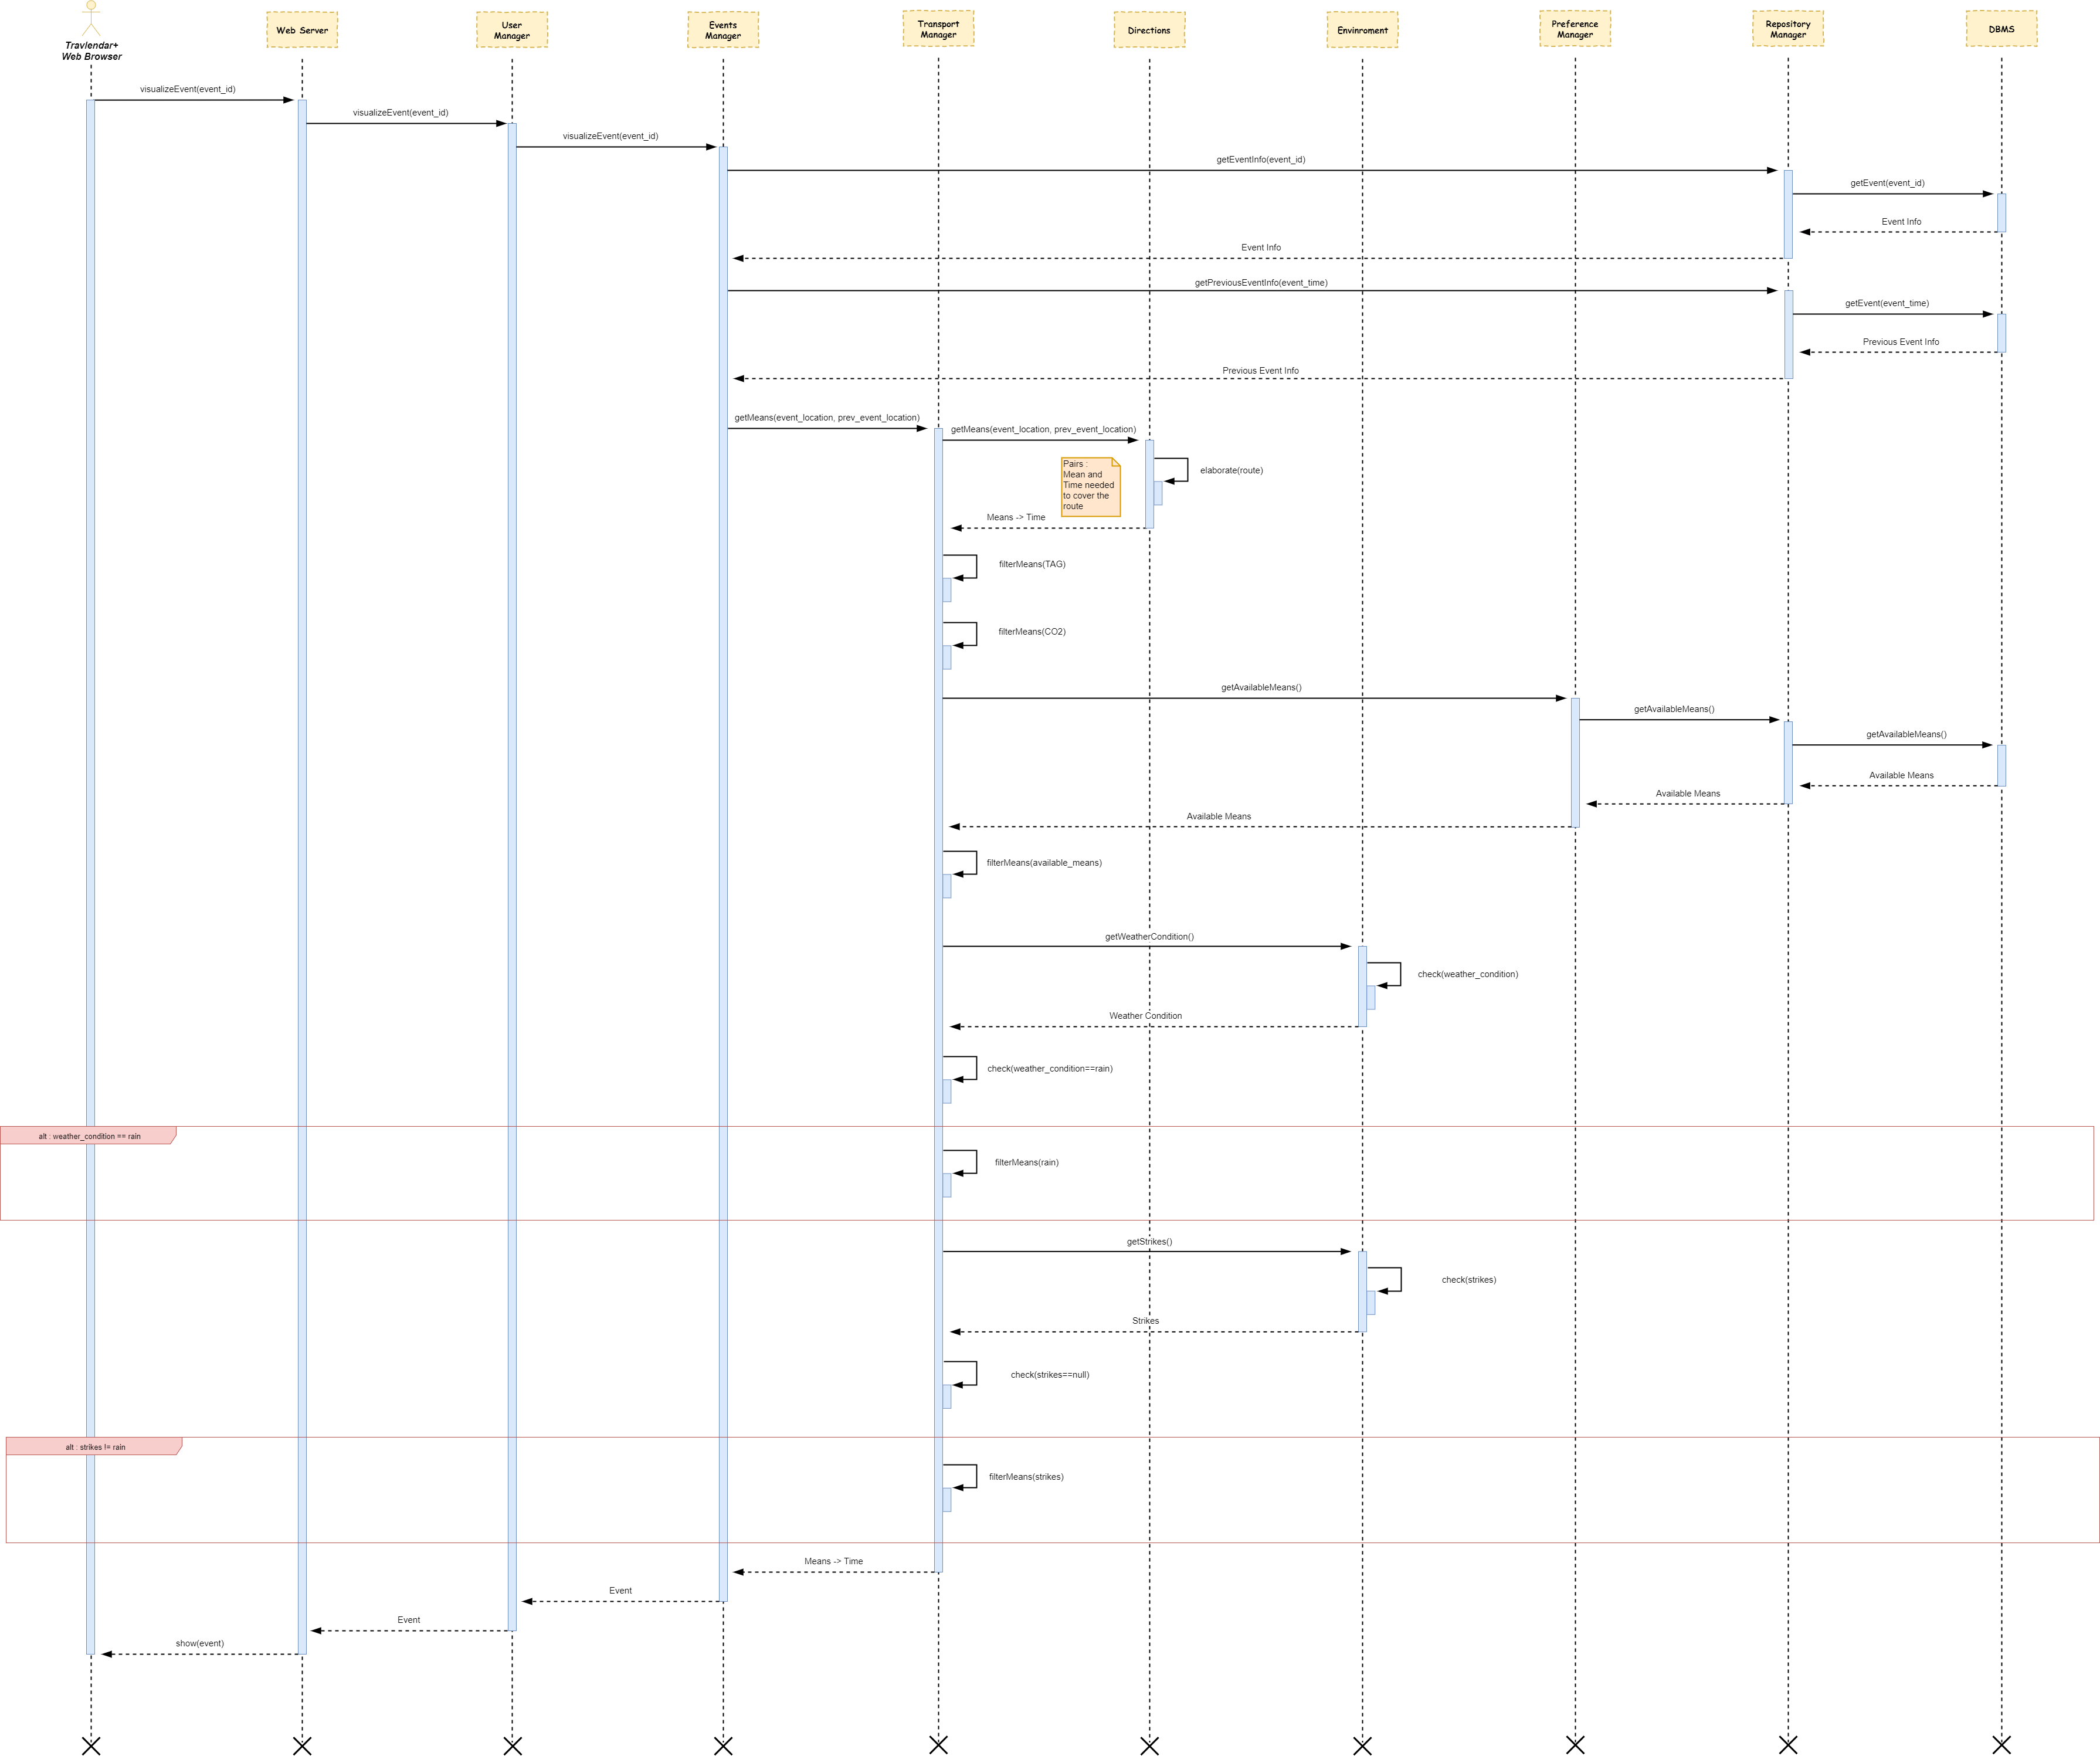
\includegraphics[scale=0.125]{Images/Runtime/Visualize_Event}
	\caption{Visualize Event Runtime View}
\end{figure}

\mysubsubsection{Visualize Directions}
This Runtime View shows a user's Visualization Directions process.\par
In order to reduce the diagram size we make a premise : the system has already checked that exists an event before the one that the user wants to get directions.\par
The Server receives the user request to show him the directions to reach a specific event. In order to do that, the Events Manager gets from the DB the information about the choosen event and the previous one. Once it receives them, asks the Directions component to elaborate the route between the given locations and finally it shows the result to the user.
\begin{figure}[H]
	\centering
	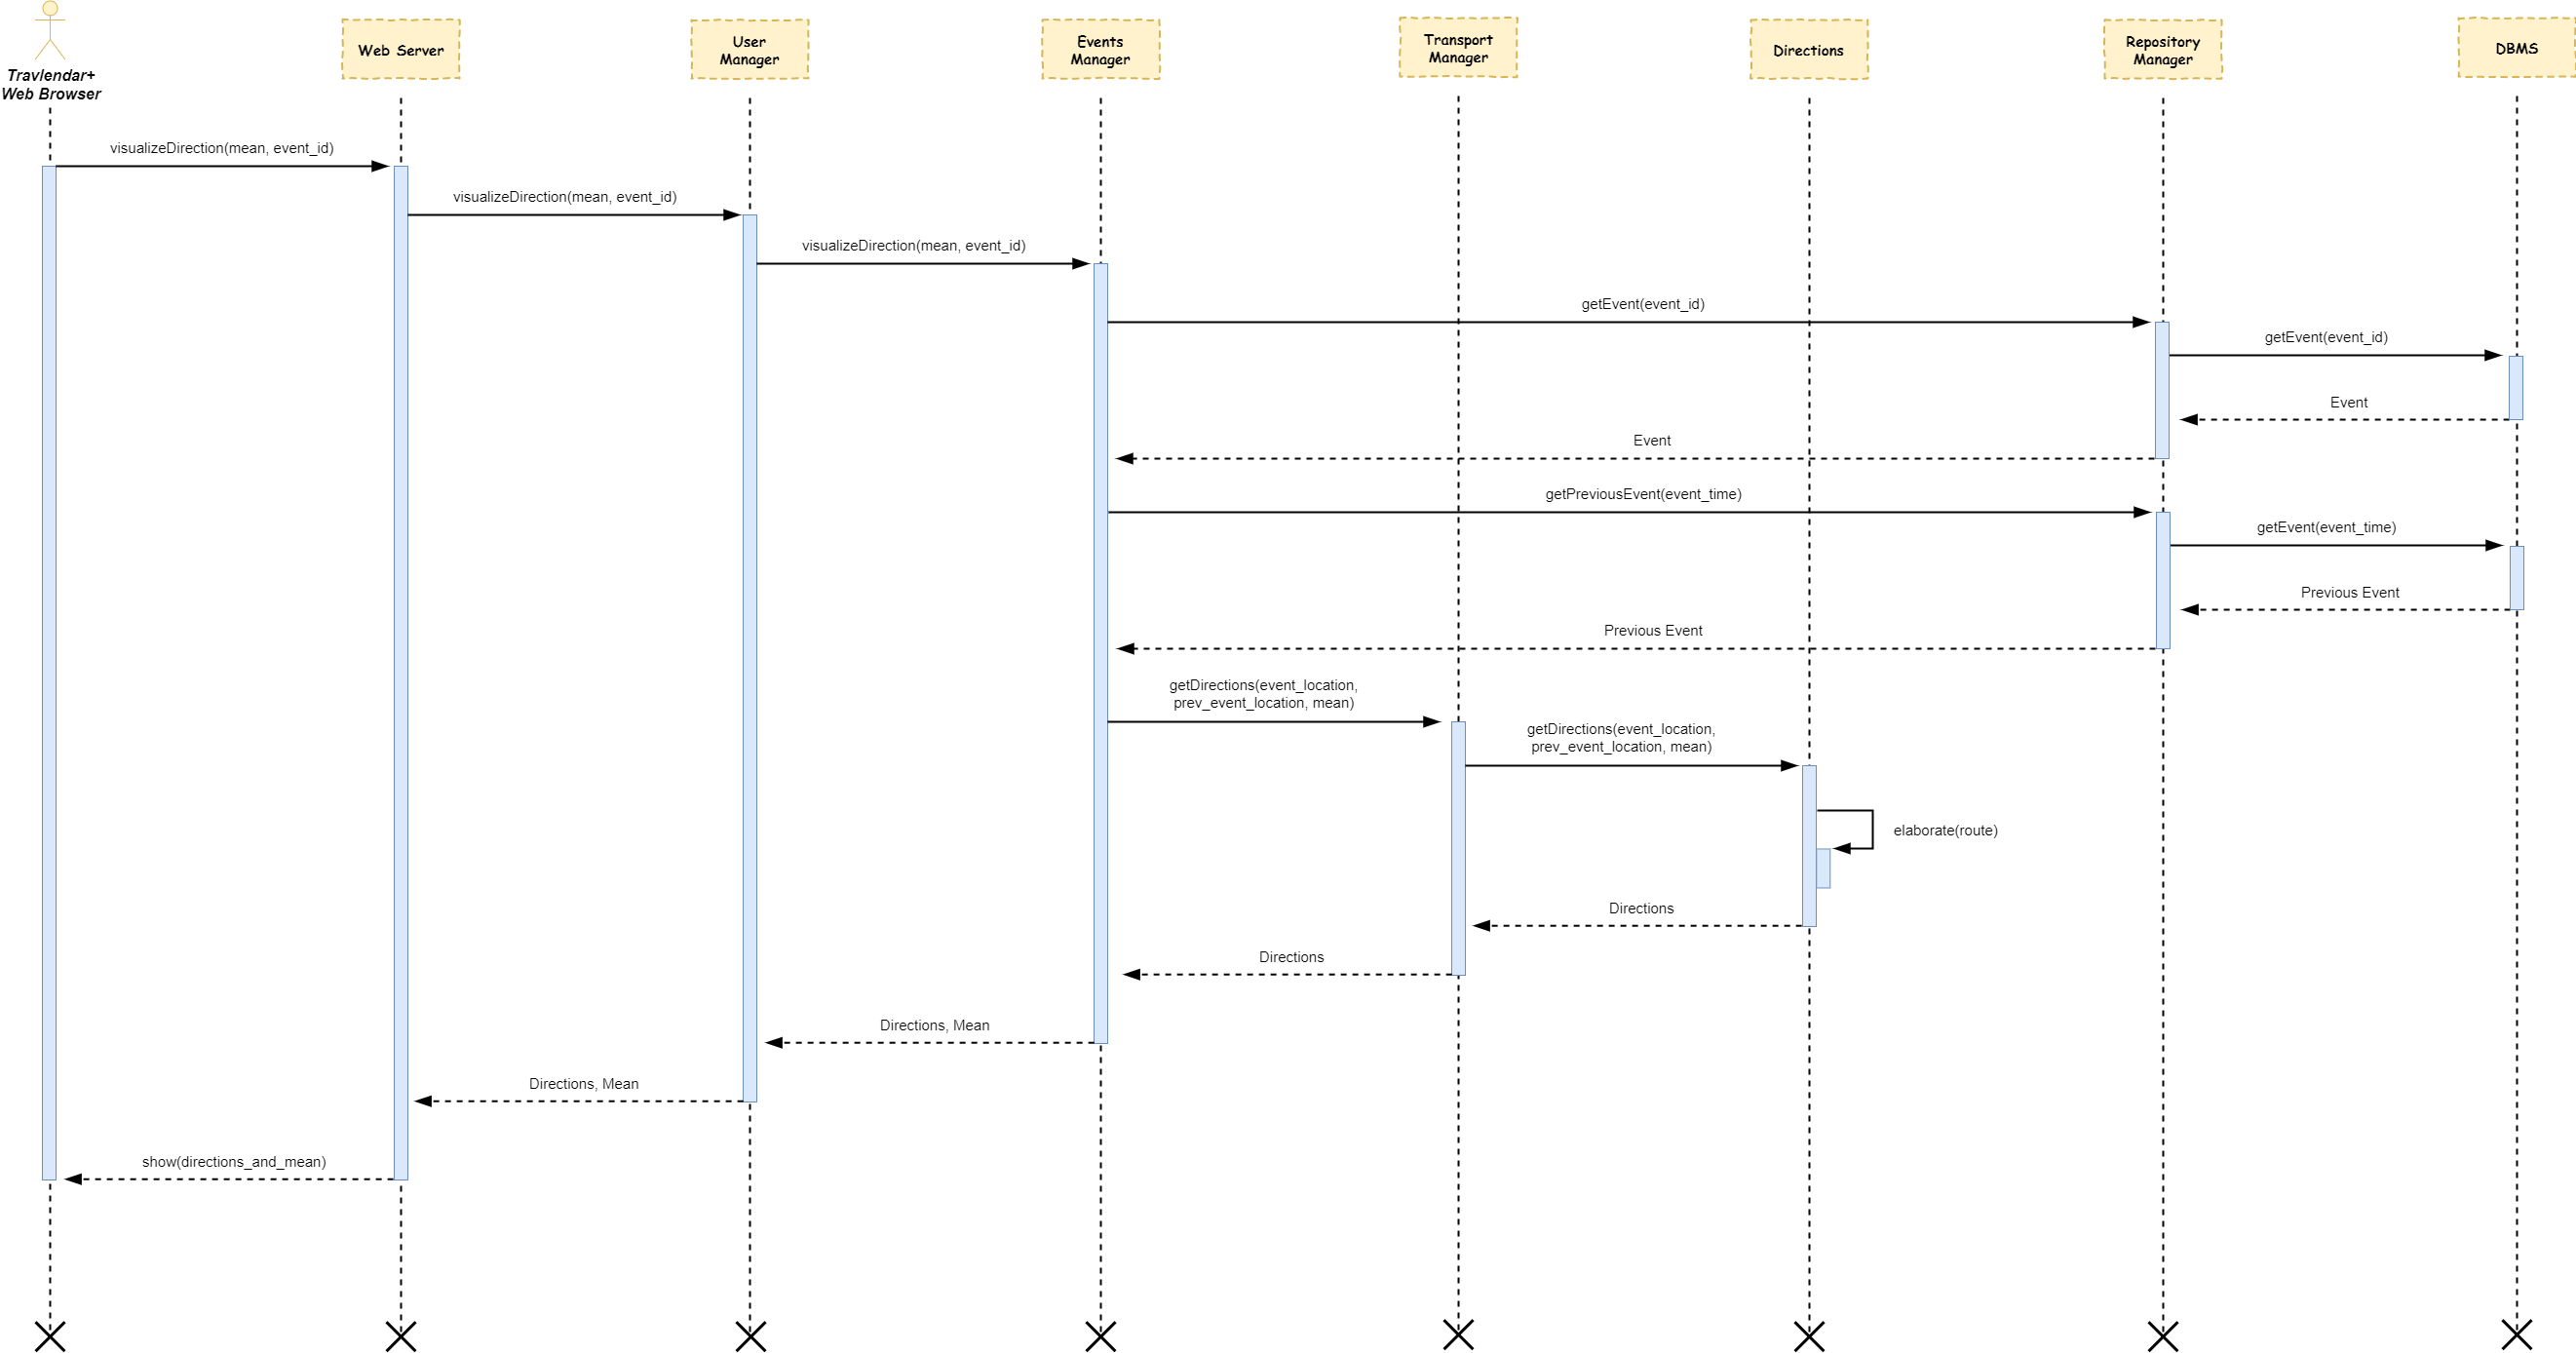
\includegraphics[scale=0.16]{Images/Runtime/Visualize_Directions}
	\caption{Visualize Directions Runtime View}
\end{figure}

\mysubsubsection{Weather \& Strike Check}
This Runtime View shows the Weather and Strike Check process.\par
In order to implement this in an efficient way we decide to create two server threads that wakes up every 24h and checks the weather conditions and the presence of strikes for the next days.\par
As seen in Add Event diagram, in the first part the user adds an event for tomorrow, just to make sure that there’s something to check for the next day.\par
At midnight the Weather thread, in the Environment component, wakes up and asks the DB for all the locations that it has to check. Once it receives them, it checks if tomorrow will rain and in that case will notify it to the user.\par
The same happens with the Strike thread.
\begin{figure}[H]
	\centering
	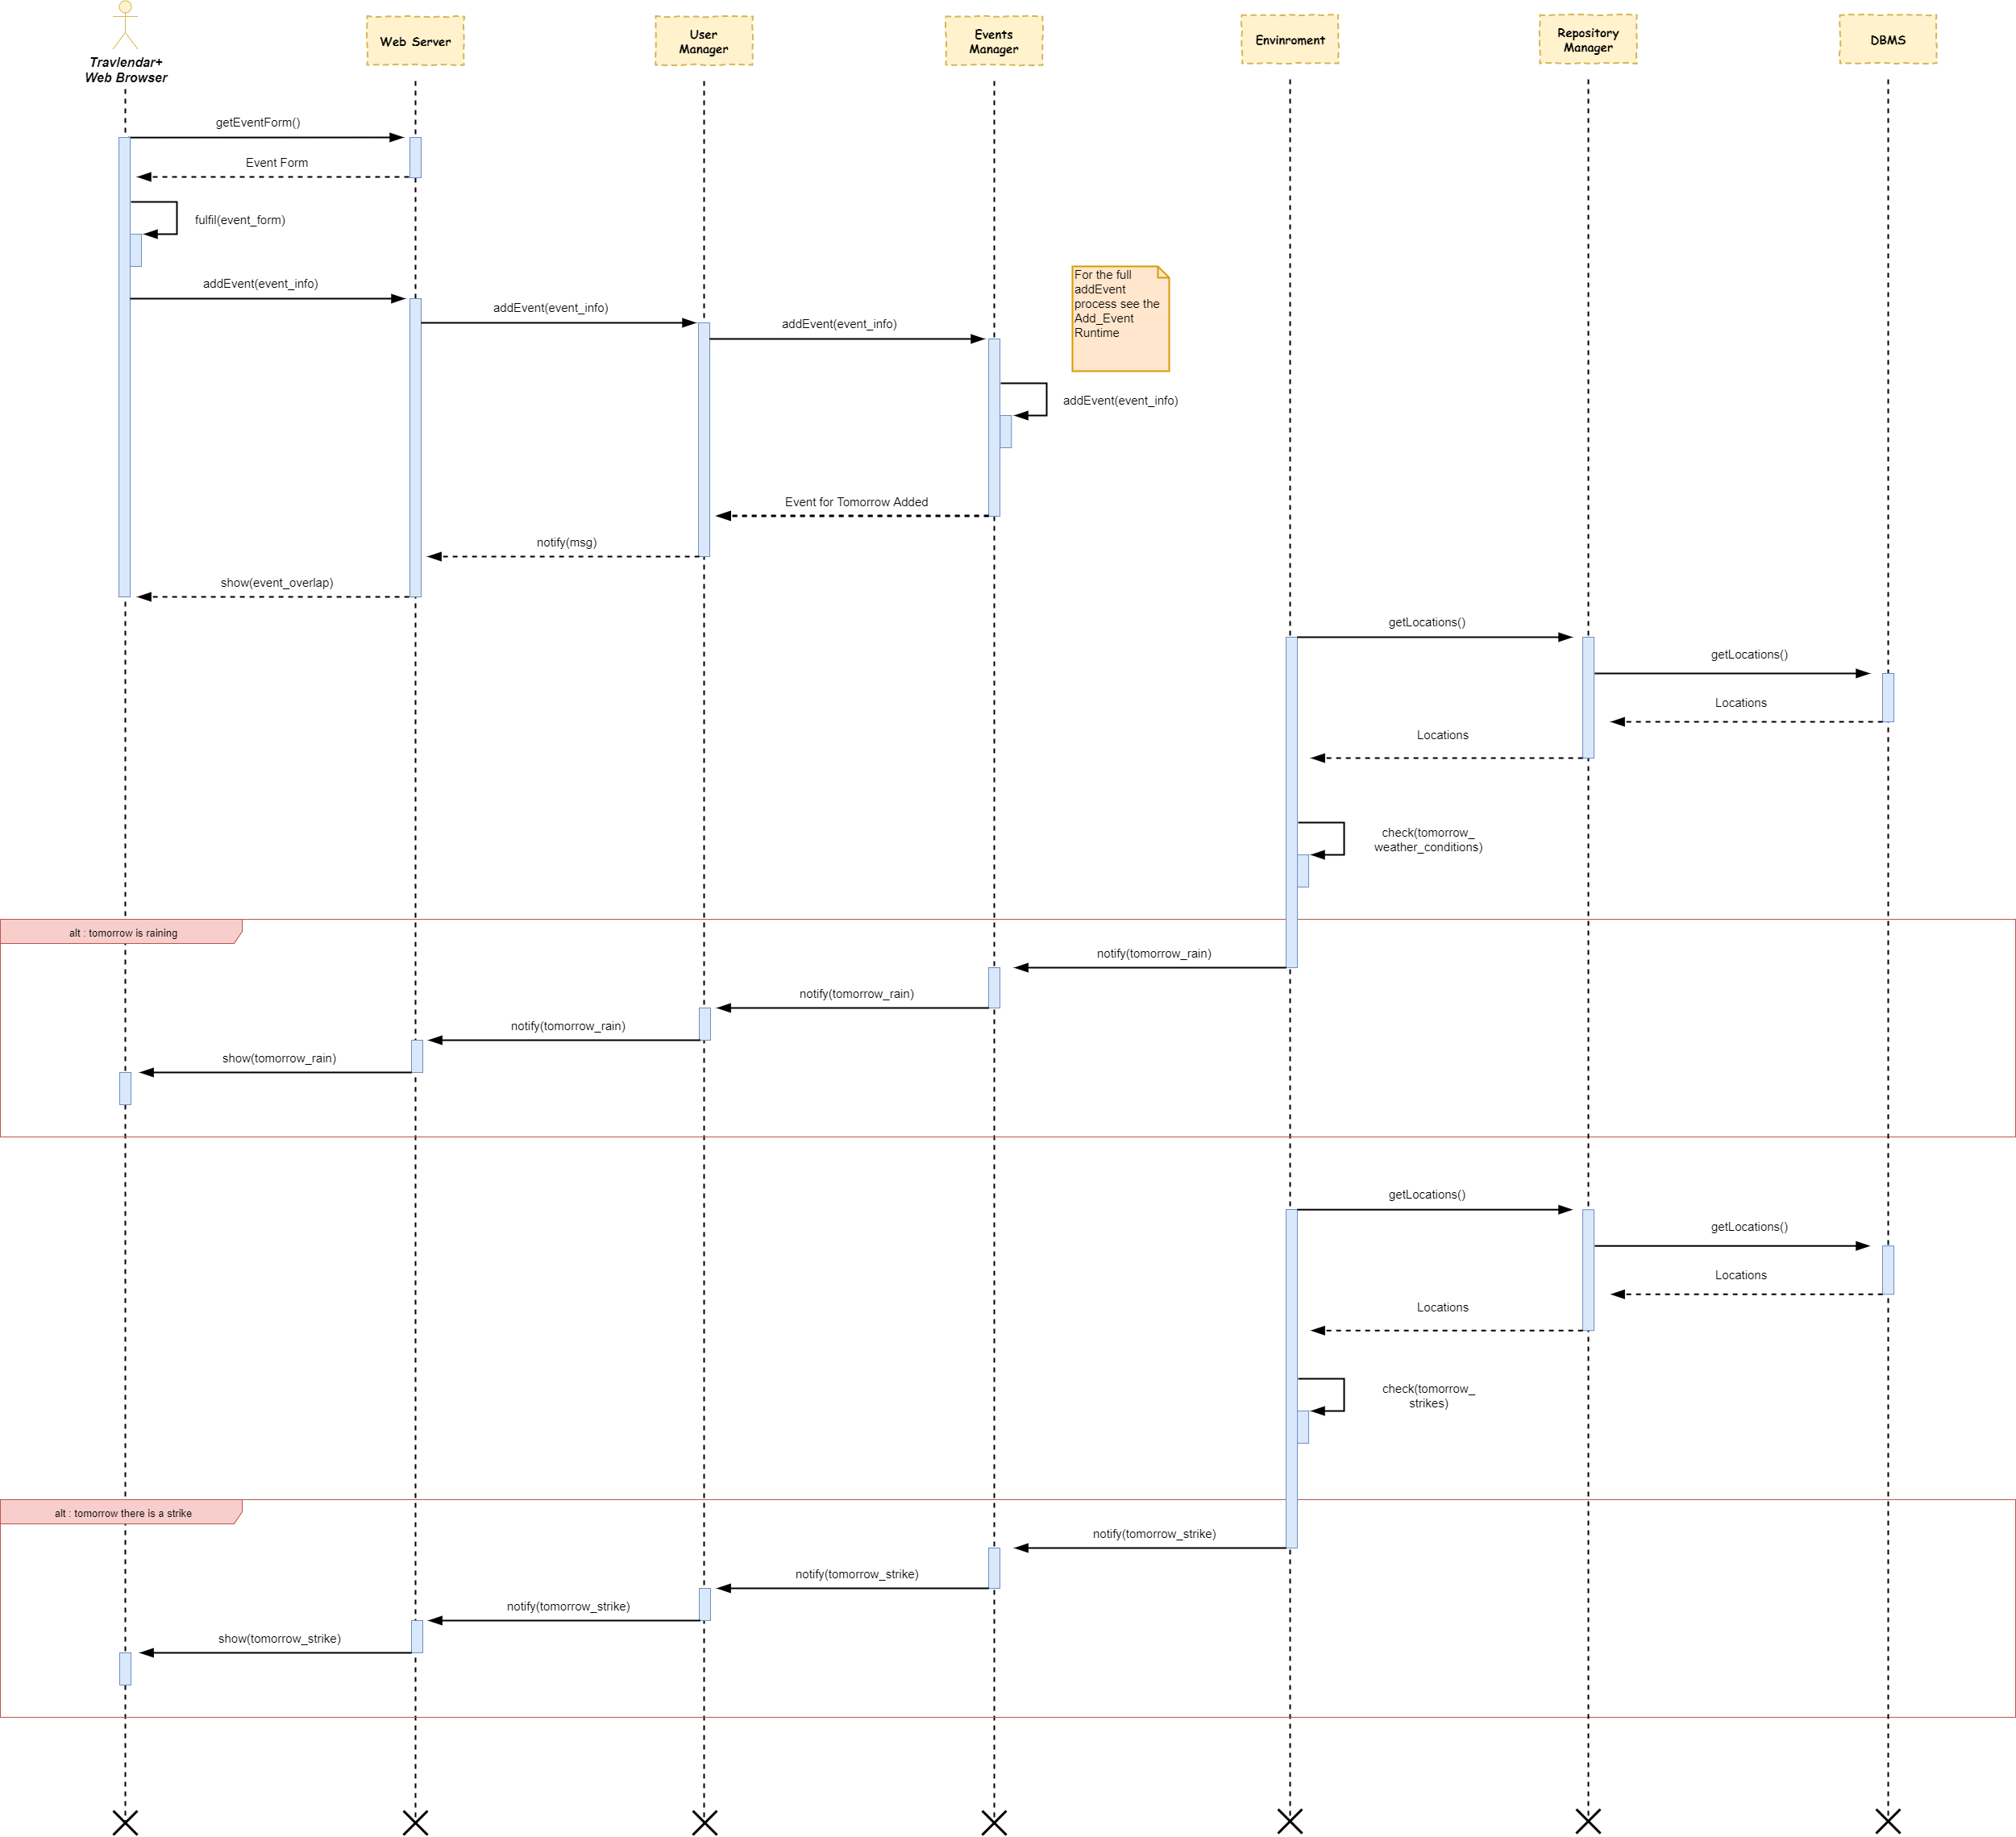
\includegraphics[scale=0.165]{Images/Runtime/Weather_Strike_Check}
	\caption{Weather \& Strike Check Runtime View}
\end{figure}

\mysubsubsection{Add Trip}
This Runtime View shows a user's Add Trip process.\par
In order to reduce the diagram size we make some premises :
\begin{itemize}
	\setlength{\leftskip}{1cm}
	\item The Overlap and Reachability checks aren’t fully showed. For more details watch the Add Event Runtime View above.
	\item The user has inserted just a departure travel, so all the checks for the travel event are executed just one time, instead of two.
\end{itemize}\par
In this diagram, the user receives a form to fulfil and to send back to the Web Server.
Once the server receives the trip\_form, it sends that to the Trip Manager, which checks if the trip is already present in the DB (get\_result!=\emph{Null}).\par
After that it has to check if the departure travel event can be added to the calendar. For performing this control, it has to ask the Events Manager to check the Overlap and the Reachability.\par
If all checks succeed Events Manager adds to the DB the travel event and Trip Manager adds the Trip.
\begin{figure}[H]
	\centering
	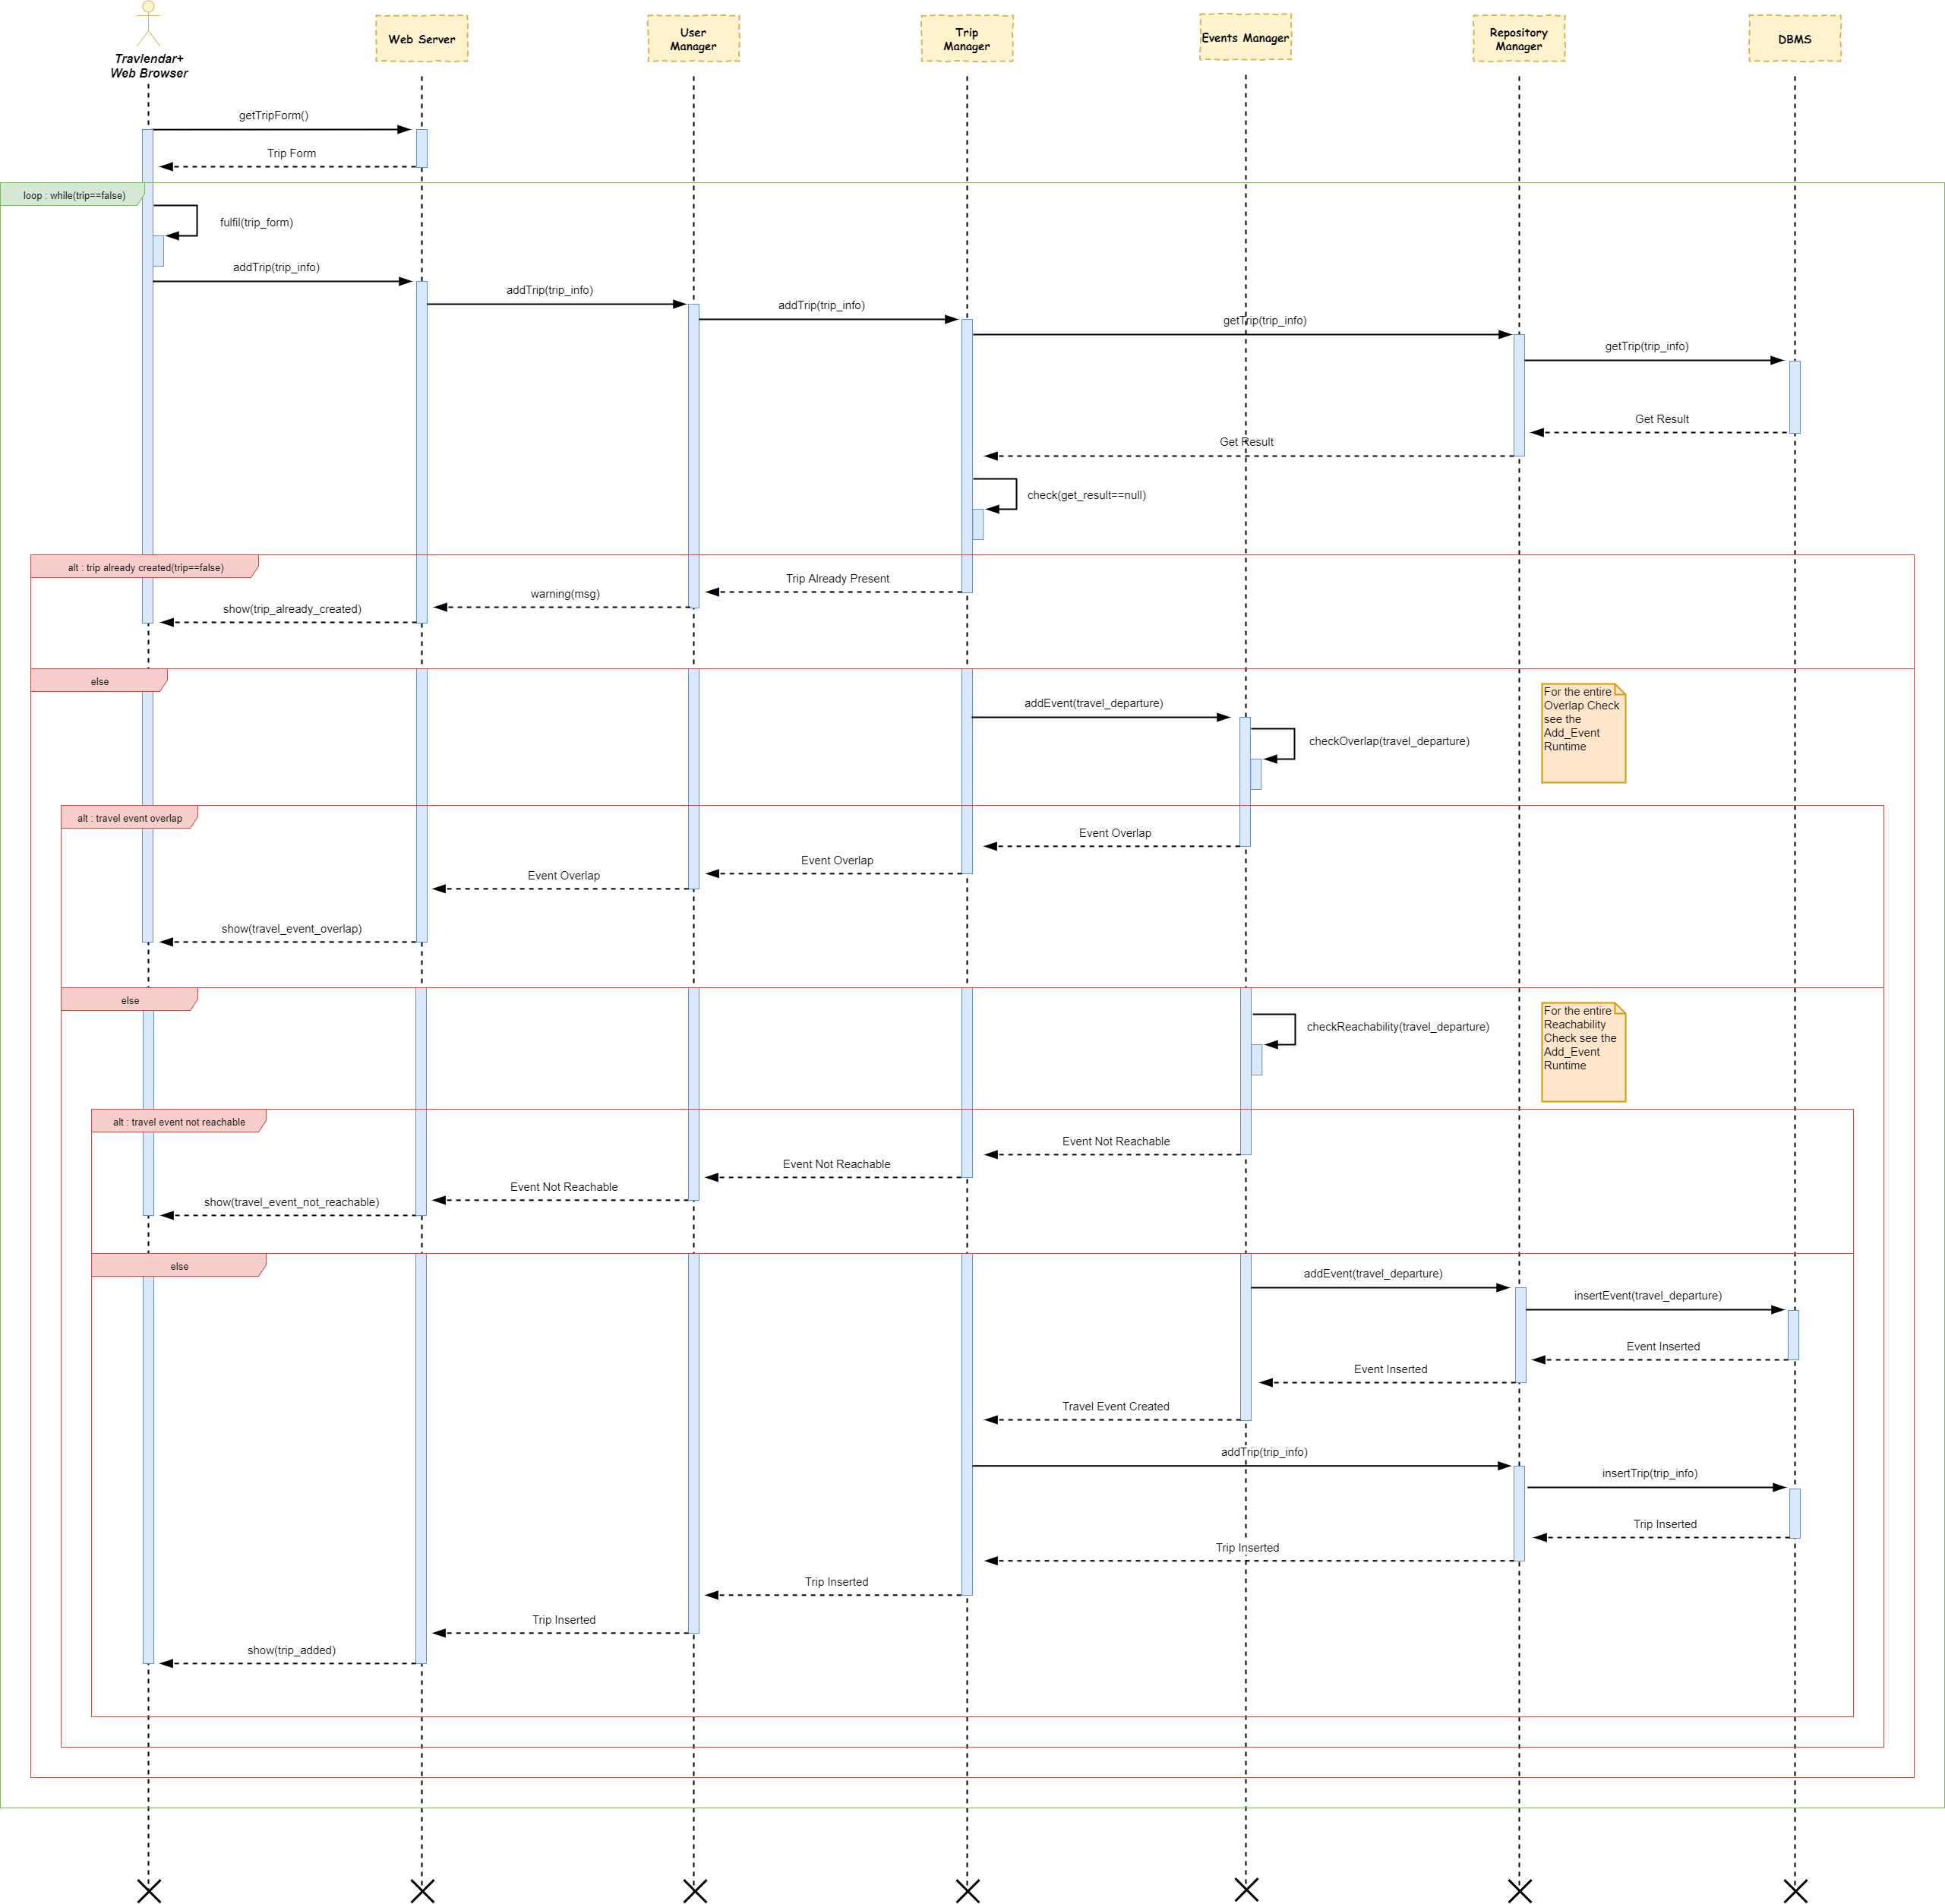
\includegraphics[scale=0.165]{Images/Runtime/Add_Trip}
	\caption{Add Trip Runtime View}
\end{figure}

\mysubsection{Selected Architectural Styles and Patterns}
Our system architecture proves to be a mix between three well known architectural styles, in particular : 

\begin{itemize}
\setlength{\leftskip}{0.5cm}
\item \emph{Client/Server Architectural style}
\item \emph{Main program with subroutines architectural style}
\item \emph{Service oriented Architectural style}
\item \emph{Event Based Architectural style}
\end{itemize}

Travlendar+ is both a web-based application and a mobile application. For the web application we will have a very thin client with the only aim of performing requests to the Business Logic through a web server.
On the other hand, the mobile application will not require an interface with the web server because it will communicate directly with the server.
\\\par
The main server will contain all the logic of the system. The main component of the logic will be the User manager. This component will perform as the Main program in the \emph{Main program with subroutines style}: it will receive the requests from the clients and call the right sub-components for accomplishing the goals related to them.
\\\par
An essential of our system business, as said in the RASD, will be to provide directions related to the precise travel means, sharing means’ position and tickets information about local and outdoor public transport. All this information will not be stored in our DBs, but they will be retrieved with API REST requests to an appropiate external services. For this goal we will use a \emph{SOA style}. 
In our system we will have a component called Transport manager that will be able to distinguish the kind of the request and it will delegate to another precise component, devoted to a certain type of external services connection, the aim of submitting it to the right external service . Once that the information has been received, its manipulation will be performed internally to the business logic of the system. In this way we will have the possibility of adding new components for incoming kind of means of transport, also personalized, in a very simple and scalable way.
\\\par
The last architectural style exploited is the \emph{Event based Architectural style}, and it is used for the notification system that will be always waiting for a particular event that, if happens, triggers a notification that is immediately sent to the right clients subscribed to the topic. 

\mysubsection{Design patterns}

\mysubsubsection{MVC}
\begin{figure}[H]
	\centering
	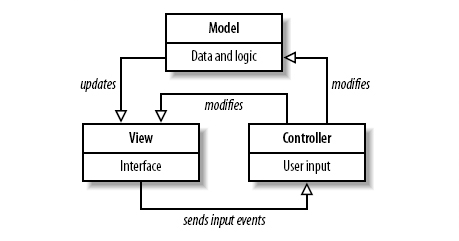
\includegraphics[scale=0.4]{Images/Patterns/MVC_Pattern}
	\caption{MVC Pattern}
\end{figure}
The Database server contains all the software’s data and constitutes the model part. The presentation layer, composed by the web-based application and the mobile application, represent the view that is released to the user. Finally the main server,  that is the business logic layer, is the control part.

\mysubsubsection{Observer}
\begin{figure}[H]
	\centering
	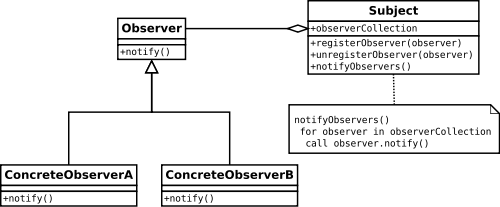
\includegraphics[scale=0.45]{Images/Patterns/Observer_Pattern}
	\caption{Observer Pattern}
\end{figure}
Our software has to be able to advise the user that he has to take a certain mean of transport for allowing him to arrive on time, that the registered season ticket is going to expire or also if a strike or bad meteorological conditions are forecasted. All these events have to be supported by a notification system. These needs will be implemented with the \emph{observe pattern}.  There will be a specific group of event listener, namely objects that extend a common abstract class. The system will have as many event listeners as is necessary and they can be added freely for future expansion. When during a process a state of interest for a listener is changed, some checks are performed and, under some particular conditions, a notification is created and sent to the user. 

\mysubsubsection{Strategy}
\begin{figure}[H]
	\centering
	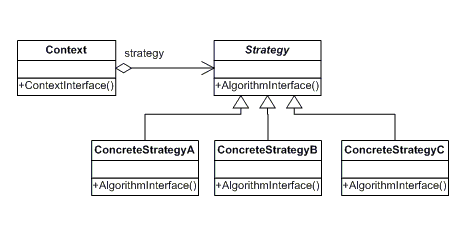
\includegraphics[scale=0.7]{Images/Patterns/Strategy_Pattern}
	\caption{Strategy Pattern}
\end{figure}
The filters applied on the data to show particular results, based on the user’s choices, for example to advise the best means of transport for a destination, will be implemented with a strategy pattern. The class that will order the results will have an instance of an abstract class that will be implemented by some concrete classes, representing different ordering strategy. In this way the system will be able to adapt its strategy runtime and it will be very simple to add new strategies creating new classes that will implement the abstract strategy class previous mentioned.

\mysubsubsection{Composite}
\begin{figure}[H]
	\centering
	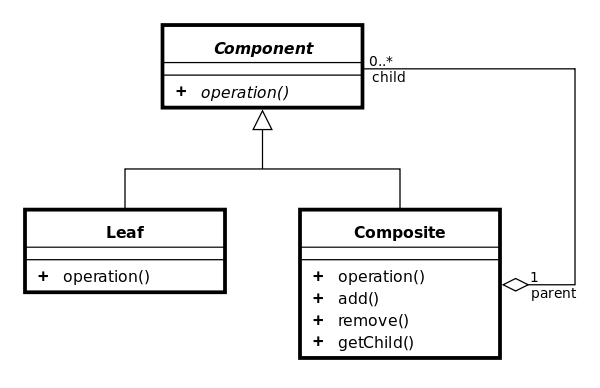
\includegraphics[scale=0.35]{Images/Patterns/Composite_Pattern}
	\caption{Composite Pattern}
\end{figure}
We will use this pattern in our system to perform, in a cleaned and elegant way, the various checks that will have to be applied on the user input. There will be a abstract class called Checker that will be extended by Composite checkers and Checkers. Each composite checker will contain one or more checkers and both implement a common interface using the \emph{check} method. The class that will have to manage a specific user input will have one or more composite checkers.
When a method that have to process the user input data, addresing them to an external service or to another component that will insert such a data in a DB, the check method of all the composite checker in such a class will be called and each composite checkers will recursively call his checker’s check method. In this way all the checks will be applied and if something is wrong, the subsequent operation will not be executed and all the possible problems linked with that will be avoided. 
Thanks to this pattern is possible to create new checkers/composite checkers very easily and to deal with complex and composite check that will be needed in future software expansions.

\mysubsubsection{Façade}
\begin{figure}[H]
	\centering
	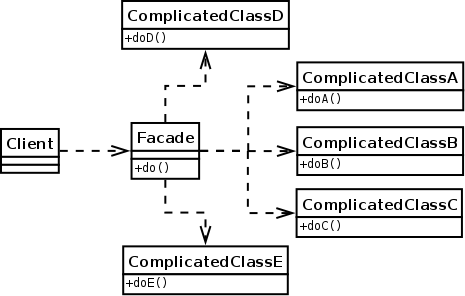
\includegraphics[scale=0.3]{Images/Patterns/Facade_Pattern}
	\caption{Facade Pattern}
\end{figure}
As guideline of our implementation, for all the complex operations that will require multiple methods calls from different classes we will use a façade pattern. In this way we will able to hide a complex logic operation within a single method call and to simplify the software maintenance for future changing needs.
